\section{What the networks do}\label{sec:networks}

\subsection{Sample complexity at $d=30$}

\Cref{tab:nstar30} and \cref{fig:curves} show the networks' learning curves against two reference learners:
\begin{itemize}
\item the NNGP kernel \cite{lee2018nngp} of the same architecture, in kernel ridge regression;
\item an Occam learner that picks the smallest junta, of up to 4 variables, consistent with the training set.
\end{itemize}
The networks sit between the two, in a specific way \status{Numerical}:
\begin{itemize}
\item \textbf{Sparse high-order targets.} Parities cost the networks 3–4$\times$ more data per extra bit: 200, 843 and 2728 samples. The Occam learner needs at most 16, 23 and 37, and the kernel fails from 3 bits on.
\item \textbf{Dense leap-1 targets.} MAJ$_9$ and the 10-bit halfspace are 3–6$\times$ cheaper for the networks than for the kernel, and out of reach of the junta learner.
\end{itemize}

\begin{table}[t]
\centering\small
\begin{tabular}{lcccccc}
\toprule
target & relevant & leap & $\nstar$ networks & $\nstar$ NNGP kernel & $\nstar$ Occam (juntas)\\
\midrule
$x_1$ & 1 & 1 & 47 & 29 & 16\\
MAJ$_3$ & 3 & 1 & 112 & 73 & 18\\
MAJ$_9$ & 9 & 1 & 263 & 1470 & --\\
random halfspace, 10 bits & 10 & 1 & 563 & 1701 & --\\
$\chi_2$, $\chi_3$, $\chi_4$ & 2, 3, 4 & 2, 3, 4 & 200, 843, 2728 & 406, --, -- & $\le$16, 23, 37\\
staircase, 5 terms & 5 & 1 & 1514 & -- & --\\
MAJ$(x_1x_2,x_3x_4,x_5x_6)$ & 6 & 2 & 1380 & 1129 & --\\
multiplexer $x_4\,?\,x_1x_2x_3:\mathrm{MAJ}_3$ & 4 & 1 & 1156 & -- & 37\\
3-term DNF & 9 & 1 & 505 & 564 & --\\
sign$(2x_1+x_2x_3+x_4x_5x_6)$ & 6 & 3 & 2205 & -- & --\\
\bottomrule
\end{tabular}
\caption{Sample complexity at $d=30$, width 128, Adam (selected targets). ``--'' means test error never reached 0.1 in the range tested ($n\le4096$ for the kernel, $n\le16384$ otherwise). The junta learner cannot represent targets with more than 4 relevant variables.}
\label{tab:nstar30}
\end{table}

\begin{figure}[t]
\centering
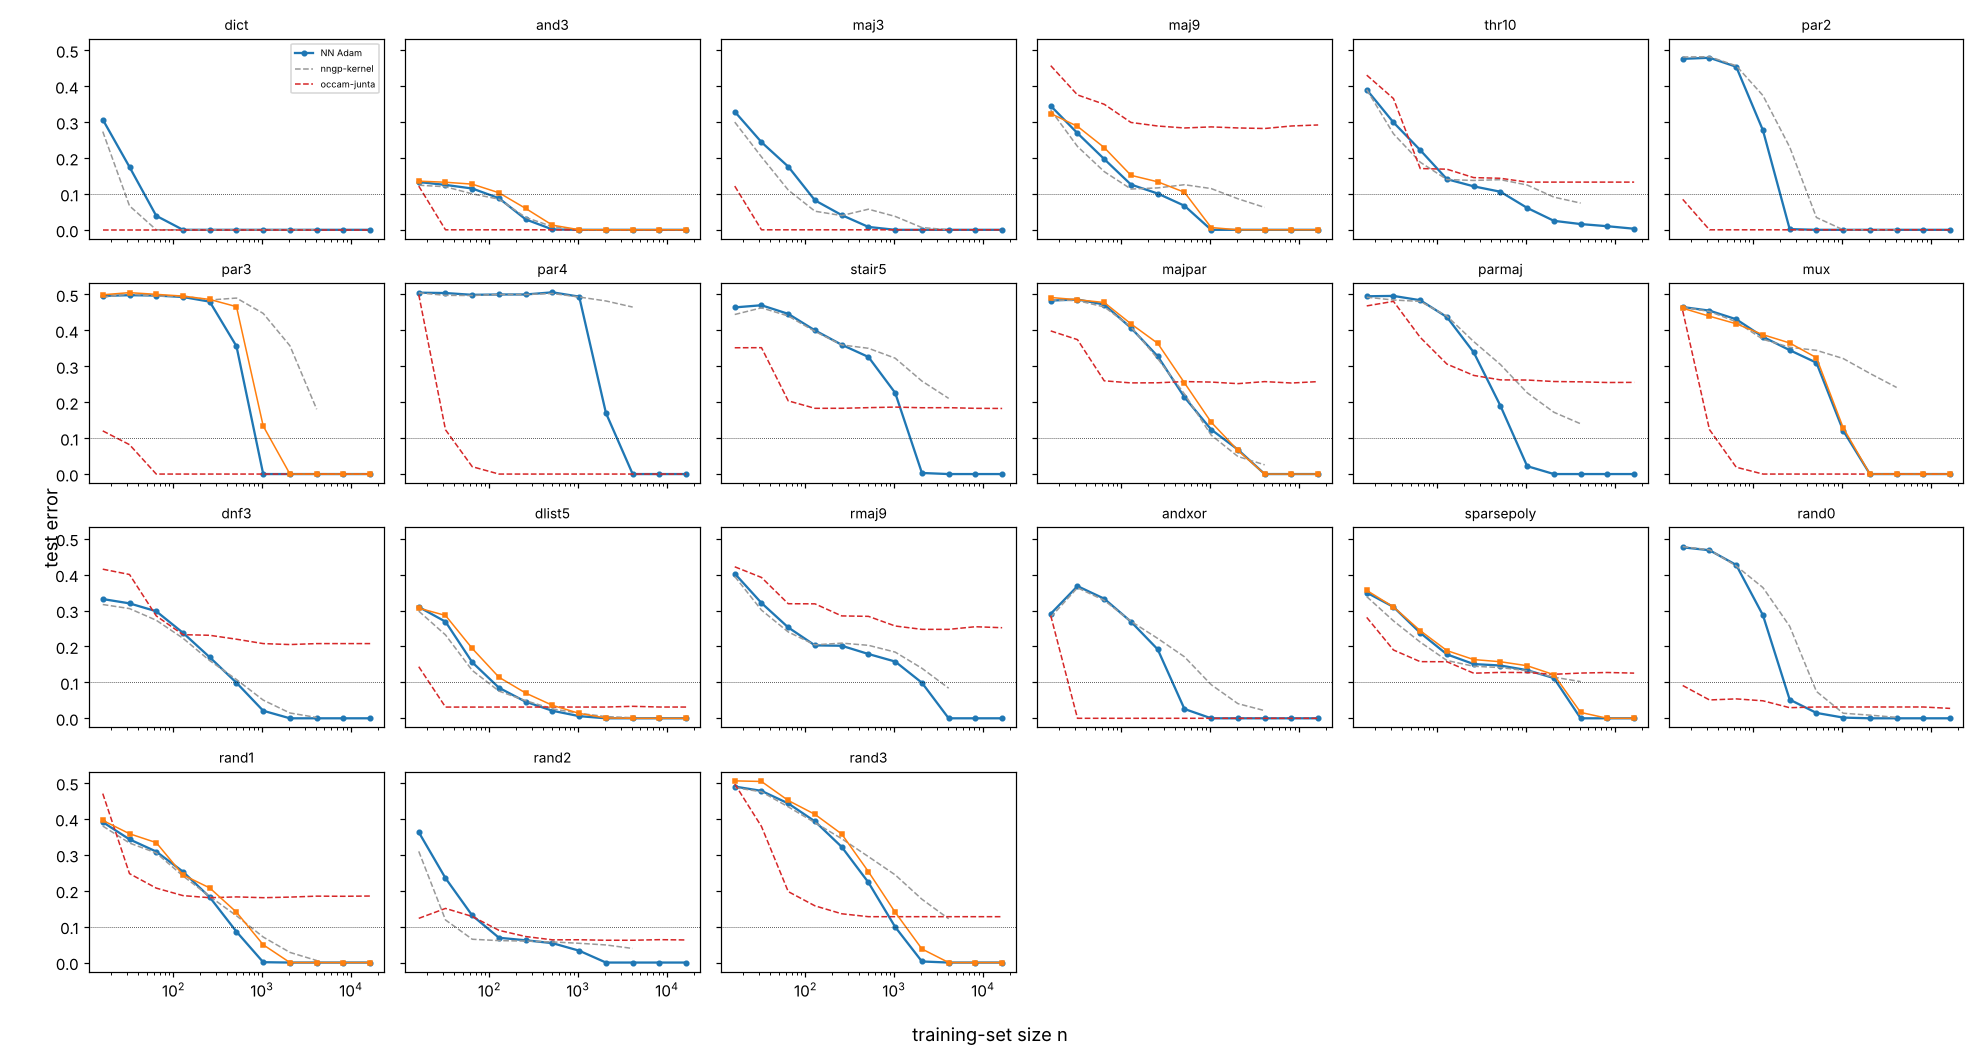
\includegraphics[width=\linewidth]{figures/nn_learning_curves.png}
\caption{Test error at the end of training against training-set size, $d=30$. Blue: Adam-trained networks (3 seeds). Orange: $\mu$P-SGD-trained networks, on the held-out targets (2 seeds). Grey dashed: NNGP kernel ridge regression. Red dashed: Occam over juntas of up to 4 variables.}
\label{fig:curves}
\end{figure}

Several further observations \status{Numerical}:
\begin{itemize}
\item \textbf{Reusing the training set saves data.} With fresh samples at every step, the networks need 12--64$\times$ their fixed-set $\nstar$: about 12800 samples for $\chi_2$, and about 32000 for $\chi_3$, the staircase, the multiplexer and MAJ of parities.
\item \textbf{Generalization is delayed near $\nstar$.} At $n=256$, $\chi_2$ fits its training set by step 200 but generalizes only at steps 7000--10000. The multiplexer, the DNF, recursive majority and AND$(x_1x_2,x_3x_4)$ show 4--40$\times$ delays at their critical $n$.
\item \textbf{Features are learned in staircase order.} On the staircase target, the network's Fourier coefficient reaches half its target value at step 100 for $x_1$, step 500 for $x_1x_2$ and $x_1x_2x_3$, and step 1000 for $x_1x_2x_3x_4$.
\item \textbf{Representation size peaks just below $\nstar$.} For the 3- and 4-bit parities, the staircase and the multiplexer, the participation-ratio rank of the second layer's kernel peaks just below $\nstar$ and collapses above it. Below $\nstar$ the networks fit the training set with many features; above it they use the target's few features.
\end{itemize}

\subsection{Dependence on the input dimension}\label{sec:dscale}

\Cref{tab:dscale} and \cref{fig:dscale} show $\nstar$ at $d=15,30,60$, and at $d=120$ for four targets \status{Numerical}. The growth with $d$ is polynomial, with an exponent that increases with the number of inputs that must be found at once:
\begin{itemize}
\item \textbf{Parities.} For 2- and 3-bit parities the exponents are $1.04$ and $1.91$ over $d=15$–$60$. On a refined grid of $n$ (quarter-octave steps), the local exponents from $d=30$ to $120$ are $1.09/1.03$ and $1.93/1.96$. Both match the CSQ rate $d^{\max(1,k-1)}$ \cite{abbe2023leap,benarous2021online}. The 4-bit parity grows like $d^{2.40}$, below $d^{3}$.
\item \textbf{Leap-1 compositions} (staircase, multiplexer) grow like $d^{1.5}$.
\item \textbf{MAJ$_9$.} Its whole learning curve is a function of $n/d$ at all four $d$, within 0.01–0.04 of a constant-free prediction from the sampling noise of the linear (Hebbian) direction (\cref{fig:dscale}b). Its apparent $\nstar$ exponent comes from where this flat curve crosses 0.1.
\end{itemize}
Occam-type laws grow like $\log d$, an effective exponent of about 0.2 over this range, and fail completely.

Training reuses a fixed sample for many epochs, so the networks are not CSQ learners in the strict sense. SQ algorithms, or gradient descent that reuses batches, can reach $d^{k/2}$ in Gaussian single-index models \cite{damian2024gaps,dandi2024reuse}. For $k\le3$ the networks here nevertheless follow the CSQ exponent; at $k=4$ they fall between the two rates.

\begin{table}[t]
\centering\small
\begin{tabular}{lccccc}
\toprule
target & $\nstar$ at $d=15$ / 30 / 60 / 120 & exponent ($15$–$60$) & CSQ $d^{k-1}$ & SQ/reuse $d^{k/2}$\\
\midrule
$\chi_2$ & 100 / 200 / 427 / 869 & 1.04 & 1 & 1\\
$\chi_3$ & 241 / 843 / 3410 / 10691$^\dagger$ & 1.91 & 2 & 1.5\\
$\chi_4$ & 508 / 2728 / 14255 / -- & 2.40 & 3 & 2\\
staircase (5 terms) & 433 / 1514 / 3487 / -- & 1.50 & -- & --\\
multiplexer & 364 / 1156 / 2848 / 5195$^\dagger$ & 1.48 & -- & --\\
MAJ$(x_1x_2,x_3x_4,x_5x_6)$ & 306 / 1380 / 3466 / -- & 1.75 & -- & --\\
MAJ$_9$ & 123 / 263 / 625 / 845 & 1.17 & -- & --\\
\bottomrule
\end{tabular}
\caption{Network sample complexity against input dimension (Adam, width 128; 3 seeds at $d=30$, 2 elsewhere). $^\dagger$On a refined (quarter-octave) $n$ grid; the factor-2 grid gives 14188 and 6524. For $\chi_4$ the 20000-step budget limits $\nstar$ at both ends of the range, so the sign of its effect on the exponent is unknown.}
\label{tab:dscale}
\end{table}

\begin{figure}[t]
\centering
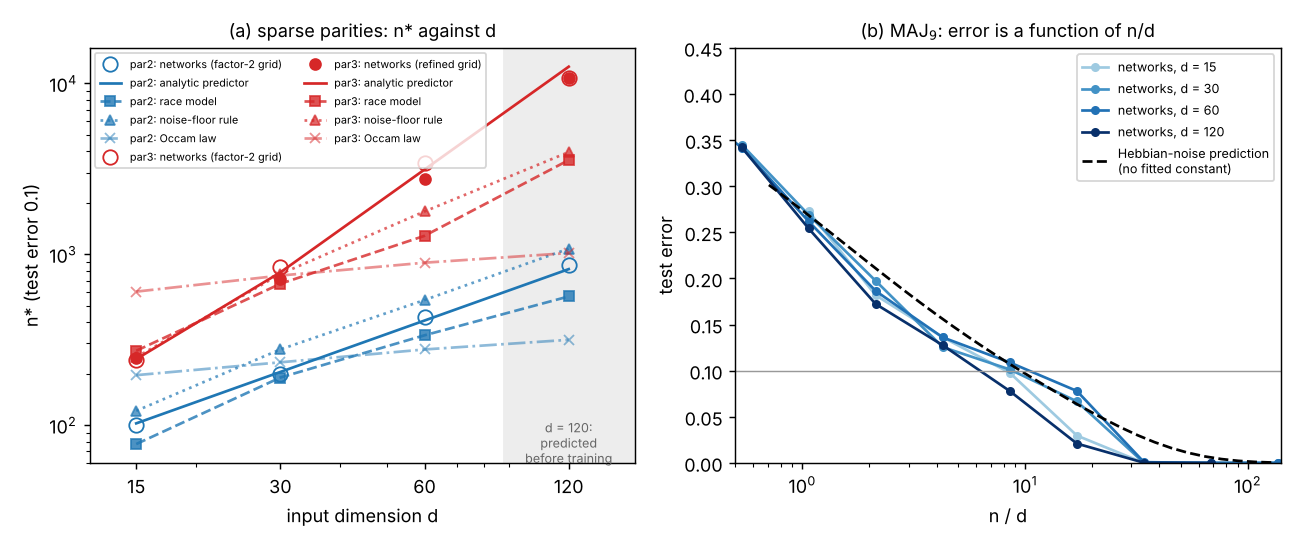
\includegraphics[width=\linewidth]{figures/understanding_dscale.png}
\caption{(a) $\nstar$ against $d$ for the 2- and 3-bit parities: networks, the analytic noise-law predictor (\cref{sec:noiselaw}), the race model, a noise-floor rule, and the Occam law. The predictions at $d=120$ (shaded) were saved before the $d=120$ networks were trained. (b) MAJ$_9$: network test error against $n/d$ at four input dimensions, and the constant-free prediction from the noise of the Hebbian direction.}
\label{fig:dscale}
\end{figure}

\subsection{Gradient descent against Occam, by leap}

Take the 26 targets, designed and random, with at most 4 relevant inputs. The ratio of the networks' $\nstar$ to the Occam-over-juntas learner's grows with the target's leap \status{Numerical}:

\begin{center}\small
\begin{tabular}{lcccc}
\toprule
leap & 1 & 2 & 3 & 4\\
targets & 14 & 8 & 2 & 2\\
median $\nstar_{\rm NN}/\nstar_{\rm Occam}$ at $d=30$ & 8.1 & 16.6 & 36 & 85\\
\bottomrule
\end{tabular}
\end{center}
Within leap 1 the spread is wide, from $1.7\times$ to $31\times$ (the multiplexer is $31\times$). The correlations along the target's greedy path matter as well as its leap. \Cref{sec:noiselaw} makes this quantitative.

\subsection{Robustness: optimizer and width}\label{sec:width}

\paragraph{SGD.} $\mu$P-SGD on the same training sets gives $\nstar$ similar to Adam's on the held-out targets: mean $|\log_2|$ ratio 0.43 \status{Numerical}. On the 3-parity, SGD needs 382, 1220 and 3562 samples at $d=15,30,60$, against Adam's 241, 843 and 3410. That is an exponent of 1.61 against 1.91. At $d=60$ both values are interpolated inside the same factor-2 step of the $n$ grid, so each exponent is uncertain by up to about $\pm0.25$, and the difference is not resolved.

\paragraph{Width.} At widths 32, 64, 128 and 256 (2 seeds; 3 at width 128) \status{Numerical}:
\begin{itemize}
\item \textbf{3-parity:} $\nstar$ does not change visibly (911, 827, 843, 873). At every width the test error is 0.28–0.47 at $n=512$ and exactly 0 at $n=1024$.
\item \textbf{4-parity:} $\nstar$ falls monotonically with width (3554, 3304, 2728, 1899), a factor of 1.9 from width 32 to 256, and has not levelled off.
\end{itemize}
This pattern does not fit a single width-dependent constant in the noise law of \cref{sec:noiselaw}, which would make the 4-parity's width effect the square of the 3-parity's. Nor does it fit a ``luckiest unit'' account. In that account the largest product of $k$ initial weights over the units would set the escape, and it predicts a width effect for the 3-parity too, since that maximum grows $1.9\times$ from width 32 to 256 at $k=3$. A guess \status{Heuristic}: the 3-parity is at its width limit by width 32, its escape carried by the bulk of the units as in mean-field theory, while the 4-parity still relies on lucky units.
